%%
%% MLSALT project dissertation template.
%%
%% Currently designed for printing two-sided, but if you prefer to
%% print single-sided just remove ",twoside,openright" from the
%% \documentclass[] line below.
%%
%%
%%   FTL, July 2016
%%   SMH, May 2010.


\documentclass[a4paper,12pt,twoside,openright]{report}

\usepackage{xcolor}
\usepackage{amsfonts}

\usepackage{hhtensor}
\usepackage{mathtools}

\newcommand{\RR}{\mathbb{R}}
\newcommand{\NN}{\mathbb{N}}
\newcommand{\m}{\vec{m}}
\newcommand{\s}{\vec{s}}
\renewcommand{\o}{\vec{o}}
\newcommand{\x}{\vec{x}}
\newcommand{\y}{\vec{y}}
\newcommand{\U}{\matr{U}}
\newcommand{\V}{\matr{V}}
\newcommand{\W}{\matr{W}}
\DeclareMathOperator*{\softmax}{softmax}

\newcommand{\todo}[1]{}
\renewcommand{\todo}[1]{{\color{red} TODO\@: {#1}}}


%%
%% EDIT THE BELOW TO CUSTOMIZE
%%

\def\authorname{Feynman T. Liang\xspace}
\def\authorcollege{Churchill College\xspace}
\def\authoremail{fl350@cam.ac.uk}
\def\dissertationtitle{BachBot: Sequence Modeling of Bach Chorales}
\def\wordcount{\todo{DO THIS}}

\usepackage{epsfig,graphicx,parskip,setspace,tabularx,xspace}
\usepackage{hyperref}

\usepackage[acronym,xindy]{glossaries}
\makeglossaries
\usepackage[xindy]{imakeidx}
\makeindex
\loadglsentries[main]{glossary}
%\newglossary{symbols}{sym}{sbl}{List of Abbreviations and Symbols}

%% START OF DOCUMENT
\begin{document}


%% FRONTMATTER (TITLE PAGE, DECLARATION, ABSTRACT, ETC)
\pagenumbering{gobble}
\pagestyle{empty}
\singlespacing
% title page information
\begin{titlepage}

\begin{center}
\noindent
\huge
\dissertationtitle \\
\vspace*{\stretch{1}}
\end{center}

\begin{center}
\noindent
\huge
\authorname \\
\Large
\authorcollege      \\[24pt]

\includegraphics{CUni3.eps}
\end{center}

\vspace{24pt}

\begin{center}
\noindent
\large
{\it A dissertation submitted to the University of Cambridge \\
in partial fulfilment of the requirements for the degree of \\
Master of Philosophy in Machine Learning, Speech, and Language Technology}
\vspace*{\stretch{1}}
\end{center}

\begin{center}
\noindent
University of Cambridge \\
Engineering Department \\
Trumpington Steet \\
Cambridge CB2 1PZ       \\
{\sc United Kingdom}    \\
\end{center}

\begin{center}
\noindent
Email: \authoremail \\
\end{center}

\begin{center}
\noindent
\today
\end{center}

\end{titlepage}

\newpage
\vspace*{\fill}

\onehalfspacing
\documentclass[dissertation.tex]{subfiles}
\begin{document}
\newpage
{\Huge \bf Declaration}

\vspace{24pt}

I \authorname of \authorcollege, being a candidate for the M.Phil in Machine
Learning, Speech, and Language Technology, hereby declare that this report and
the work described in it are my own work, unaided except as may be specified
below, and that the report does not contain material that has already been used
to any substantial extent for a comparable purpose.

\vspace{24pt}
Total word count: \wordcount

\vspace{60pt}
\textbf{Signed}:

\vspace{12pt}
\textbf{Date}:


\vfill

This dissertation is copyright \copyright 2016 \authorname.
\\
All trademarks used in this dissertation are hereby acknowledged.



\newpage
\vspace*{\fill}
\end{document}

\singlespacing
\newpage
{\Huge \bf Abstract}
\vspace{24pt} 


This is the abstract. Write a summary of the whole thing. Make 
sure it fits in one page. 


\newpage
\vspace*{\fill}


\pagenumbering{roman}
\setcounter{page}{0}
\pagestyle{plain}
\tableofcontents
\printglossary[title=Notation and Abbreviations]
\listoffigures
\listoftables

\onehalfspacing

%% START OF MAIN TEXT

\chapter{Introduction}
\pagenumbering{arabic}
\setcounter{page}{1}

% This is the introduction where you should introduce your work.  In
% general the thing to aim for here is to describe a little bit of the
% context for your work --- why did you do it (motivation), what was the
% hoped-for outcome (aims) --- as well as trying to give a brief
% overview of what you actually did.

% It's often useful to bring forward some ``highlights'' into
% this chapter (e.g.\ some particularly compelling results, or
% a particularly interesting finding).

% It's also traditional to give an outline of the rest of the
% document, although without care this can appear formulaic
% and tedious. Your call.

\gls{fn}

\gls{fncon}

While deep learning has revolutionized computer vision and natural language
processing, its applications to other domains are still emerging. This
dissertation is concerned with the applications of deep learning to a new
problem domain: music scores.

In this work, we investigate how sequence probability models parameterized by
deep recurrent neural networks can be used as generative models over scores of
music. Such a model has a variety of applications within computational music
theory. The aim of this work is to investigate applications on two particular
tasks: melody harmonization and automatic composition.

Every aspiring music theorist is at some point tasked with composing simple
pieces of music in order demonstrate understanding of the harmonic rules of
Western classical music. These pedagogical exercises often include
harmonization of chorale melodies, a task which is viewed as sufficiently
constrained to allow a composer's skill to be judged. A generative model
for music scores can be applied to this task by conditioning on the melody
line and sampling the conditional distribution for possible harmonizations.

A more difficult task is automatic composition, where the composer is tasked
with producing an original composition of a particular musical style. The open
nature of this task enables a composer to simultaneously demonstrate their
creativity along with understanding of music theory. However, this lack of
constraints and loose definition of musical style makes it more difficult to
evaluate the quality of the output. To apply a generative model towards this
task, we can train the model to assign larger probability mass to stylistically
similar scores and then sample the model to generate a novel composition.

While our modeling framework is capable of modeling any MIDI-encodeable music
score, we focus our study on chorales by Johann Sebasian Bach. These provide
a relatively large corpus by a single composer, are well understood by music
theorists, and are routinely used when teaching music theory.
The aim is to build an automatic music composition system capable of imitating
Bach's compositional style on both harmonization and automatic composition tasks.

We will examine how design decisions made when constructing probability models
over music affect the musical characteristics of generated samples, investigate
practical matters encountered with parallel training and sampling across
multiple GPUs, and benchmark how well our final system performs on human test
subjects.

\chapter{Background}

% A more extensive coverage of what's required to understand your
% work. In general you should assume the reader has a good undergraduate
% degree in computer science, but is not necessarily an expert in
% the particular area you've been working on. Hence this chapter
% may need to summarize some ``text book'' material.

% This is not something you'd normally require in an academic paper,
% and it may not be appropriate for your particular circumstances.
% Indeed, in some cases it's possible to cover all of the ``background''
% material either in the introduction or at appropriate places in
% the rest of the dissertation.

Algorithmic composition is the application of a well-defined algorithmic
procedure to compose music.

An interesting question regarding creativity: if an algorithm faithfully reproduces
an artist's creative process, what is the difference between music produced by the artist
and music produced by the algorithm?


\section{Music theory}

A score of music is represented using a sequence of notes. Each note represents
a pitch (i.e.\ frequency) and duration (i.e.\ time interval).

When discussing pitches, it is common to refer to the difference between two
pitches as \textbf{pitch interval}s. One of the most fundamental pitch intervals is the
\textbf{octave} defined to be the interval between a frequency and its double.

While in theory an uncountable number of pitches are available, the tuning
system utilized by a piece of music oftentimes restricts the number of
available pitches. Western music commonly uses \textbf{twelve-tone equal
temperament} (12-TET) tuning, which divides an octave into 12 pitch classes
all equally spaced on a logarithmic scale. The interval between two adjacent
pitch classes (i.e. 1/12th an octave on log-scale) is called a \textbf{half step}
and two half steps are called a \textbf{whole step}

Tonal music is characterized by the prevalence of one pitch class (the
\textbf{tonic} around which the melody and harmony are built. A basic concept
within tonal music is the \textbf{scale} which defines a subset of pitch classes
that are ``in key'' with respect to the tonic. Two fundamental scales are the
major (with step pattern whole-whole-half-whole-whole-whole-half) and minor
scales (whole-half-whole-whole-half-whole-whole). The choice of tonic and scale
is referred to as the \textbf{key}and a change in key during a piece is called a
\textbf{modulation}Many musical phenomena such as stability, expectation, and
resolution can be attributed to tonal characteristics.

Note that while 12-TET restricts the possible intervals between notes, it does
not define an absolute reference pitch frequency. This degree of freedom gives
rise to transposition invariance: a score of music can be offset by a constant
pitch interval without affecting its tonal characteristics. For practical
performance purposes, the general tuning standard in modern times tunes the ``A''
note directly above ``middle C'' to 440 Hz (A440).

The \textbf{tempo} of a piece refers to its speed or pace and is measured by beats
per minute. In 4/4 time signature, a \textbf{quarter note} or \textbf{crotchet} denotes
the time interval between two beats. In addition to pitch quantization,
durations are also commonly quantized to subdivisions and multiples of a
crotchet.

\subsection{Notation}

We consider note duration, time, and velocity. We neglect changes in timing
(e.g. ritardandos), dynamics (e.g. crescendos), and stylistic notations (e.g.
accents, staccatos, legatos).

\emph{Piano roll} music transcriptions are quantized both in time ($t \in T$)
and note frequencies ($n \in N$). frequencies quantized to a piano roll.
\todo{Motivate quantization with Western music}.

We can represent a piano roll transcription as a high-dimensional vecctor
$X_{t,n} \in \RR^{|T| \times |N|}$ where $X_{t,n}$ denotes the note
velocities for note $n$ at time $t$.

\chapter{Related Work}

%\subsubsection{Psychoacoustic Features and Gray Codes}

% This chapter covers relevant (and typically, recent) research
% which you build upon (or improve upon). There are two complementary
% goals for this chapter:
% \begin{enumerate}
%   \item to show that you know and understand the state of the art; and
%   \item to put your work in context
% \end{enumerate}

% Ideally you can tackle both together by providing a critique of
% related work, and describing what is insufficient (and how you do
% better!)

% The related work chapter should usually come either near the front or
% near the back of the dissertation. The advantage of the former is that
% you get to build the argument for why your work is important before
% presenting your solution(s) in later chapters; the advantage of the
% latter is that don't have to forward reference to your solution too
% much. The correct choice will depend on what you're writing up, and
% your own personal preference.


\section{RNNs}

\begin{enumerate}
    \item Bidirectional RNNs
        \begin{figure}[htpb]
            \centering
            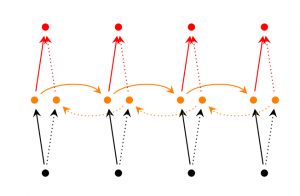
\includegraphics[width=0.8\linewidth]{Figures/bi-rnn.png}
            \caption{\todo{Redraw}}
        \end{figure}
        Cannot be sampled, but if the source sequence is given can run FW and BW LSTMs
        to obtain $\s^{FW}$ and $\s^{BW}$ then $\o_t = \softmax(V [\s^{FW}_; \s^{BW}_t])$
    \item Deep RNNs
        \begin{figure}[htpb]
            \centering
            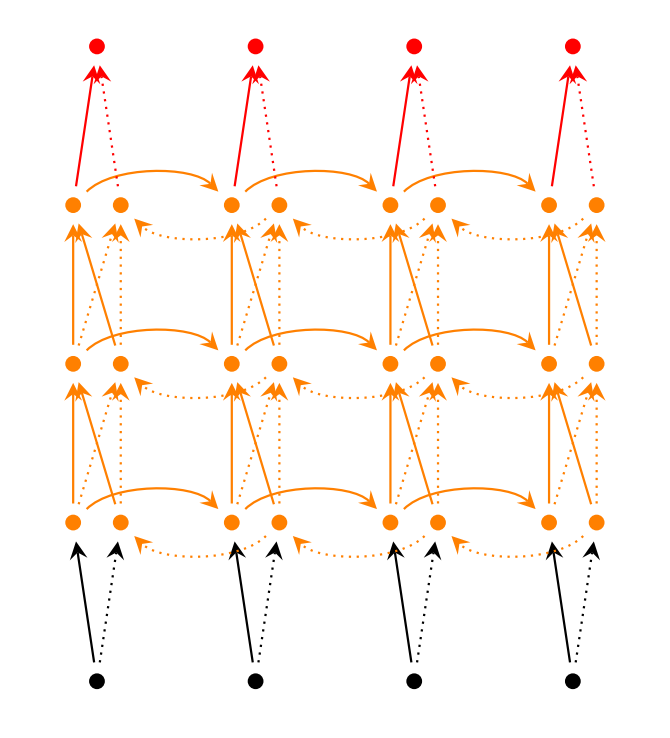
\includegraphics[width=0.8\linewidth]{Figures/deep-rnn.png}
            \caption{\todo{Redraw}}
        \end{figure}
        Outputs of one LSTM are used as inputs to the next; more layers $\implies$
        greater representational power, hierarchical representation learning?
    \item LSTMs
        \begin{enumerate}
            \item Memory is called \emph{cells}
        \end{enumerate}

    \item LSTM Variants: GRUs have fewer parameters (U and W are smaller) and
        thus may train a bit faster or need less data to generalize
\end{enumerate}

\subsection{RNN-RBM}
An alternative design is to have the RNN output the entire chord at teach time.
This is appealing because the steps between successive RNN applications
correspond to units of time. Additionaly, the emission distribution's parameterization
can be used to restrict the number of simultaneous parts.

In a RNN-RBM, the hidden state is used to compute the parameters for a restricted Boltzmann
machine at each timestep. The RBM parameterizess a multivariate categorical distribution,
which can be either over the four parts or the entire piano roll.

\chapter{Data}

We use a corpus of Bach chorales provided by \texttt{music21}. The chorales are
arranged by the Bach-Werke-Verzeichnis (BWV) numbering system, which is one of
the best known and widely used catalogues of Bach's compositions.

Each chorale has four parts and are structured such that the melody is in
the Soprano part and the remaining parts harmonize the melody.

\section{Preprocessing}

We transpose all scores with major key signatures to C major and minor key
signatures to A minor. Due to transposition invariance of 12-TET, this does
not alter the tonal properties of the music.

We represent musical scores using a piano roll representation. Firstly, time is
discretized into constant timestep frames. For each frame, a set of (note, tie)
pairs representing which a note's pitch and whether it is tied
(continuing a note from the previous frame) or newly played notes.

\begin{enumerate}
    \item Transpose to Cmaj/Amin
    \item Strip all dynamics info
    \item Restrict to 4/4
\end{enumerate}

\chapter{Sequence probability modelling}

Generating a "Bach-like" piece of music can be understood as drawing a random
sample from a distribution over musical scores which is statistically similar
to Bach's own compositions. Thus, we interpret the problem as one of
\emph{categorical sequence modeling}.

This type of problem has been well studied. In speech recognition, language
models parameterizing distributions over sentences are used as priors to refine
transcriptions.

However, since our model has to be able to generate Bach, we must be able to
sample from it. This rules out a broad class of sequence models, including
back-off N-grams and other interpolated language models.

Fortunately, low order N-grams and standard HMM-based models are sampleable and
thus can be used as baselines.

\section{Feedforward neural networks}

Increasing context window size is not always a good solution:
\begin{itemize}
    \item Too small $\implies$ no long-term dependencies captured
    \item Not all $N$-grams observed $\implies$ need back-off and discounting
\end{itemize}

How do we handle variable length inputs?

\section{Recursive neural networks}

Carry memory $s_t$ through time $t$, ``summary of infinite context duration
i.e.\ all previously processed data''

Share weights $\matr{U}, \matr{V}, \matr{W}$ over $t$ since performing same
task at each time i.e.\ modeling $P(o_t | s_t, x_t) = \softmax(V s_t)$.

\begin{figure}[htpb]
    \centering
    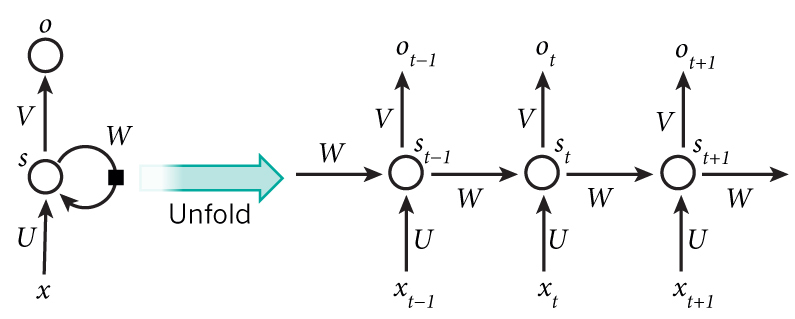
\includegraphics[width=0.8\linewidth]{Figures/rnn.jpg}
    \caption{\todo{Redraw in xy}}
\end{figure}

\begin{align}
    \s_t &= f(\U \x_t + \W \s_{t-1}) \\
    \o_t &= \softmax( \V \s_t)
\end{align}

$f$ is usually $\tanh$ or ReLU.

\begin{enumerate}
    \item Memory/state $\s_t$ summarizes ALL previous information
    \item $\U, \V, \W$ parameters are shared across all $t$. Reflects
        that the same task is being performed at each input i.e.\
        invariance over time. Reduces number of parameters.
\end{enumerate}


RNNs are a sequence model similar to HMMs in that they model the conditional
distribution of next frames given the previous context. However, RNNs additionally
pass along "hidden state" which summarizes contextual information from a potentially
infinite context window.

In practice, it is observed that the hidden state does not capture long range
dependencies well and tend to suffer from vanishing/exploding gradient during
training. LSTMs are an improved RNN architecture which solve both of these
problems by introducing gates on the inputs, hidden state, and outputs. GRUs are
a variation of LSTMs which ties the weights to the input and forget gates.

\begin{enumerate}
    \item Language modeling
        \begin{enumerate}
            \item Model $P(\m), \m \in V^T, T \in \NN$
            \item Train to predict the distribution of the next note in the
                melody i.e.\ $\o_t = P(\m_t | \m_{1:t-1})$
            \item $\m_{t-N:t-1}$ is given explicitly as input $\x_t$ and
                $\s_{t}$ captures information from before $t-N$
            \item See \cite{Martens2011}, \cite{Mikolov2011}, \cite{Mikolov2010}
        \end{enumerate}
    \item Machine translation
        \begin{enumerate}
            \item~\\
                \begin{figure}[htpb]
                    \centering
                    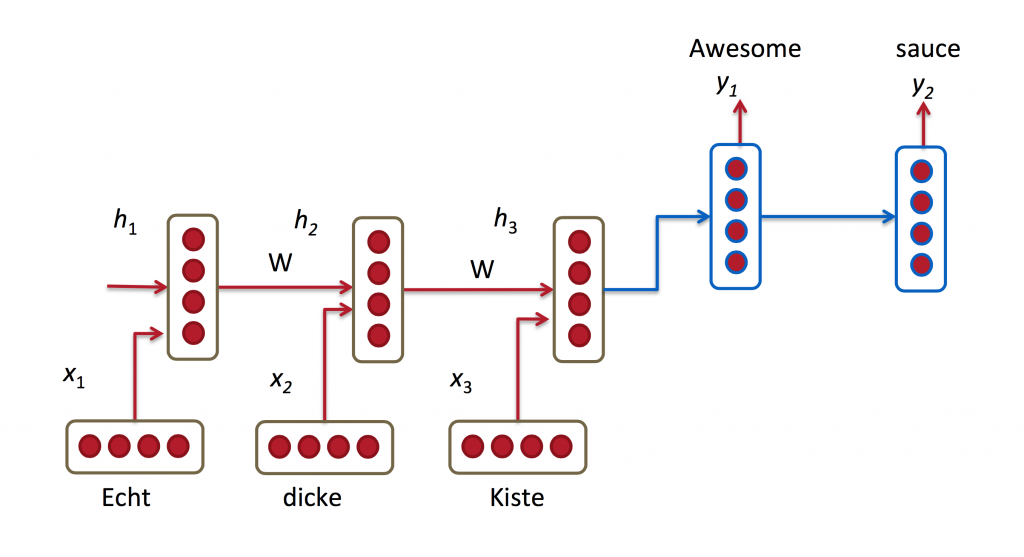
\includegraphics[width=0.8\linewidth]{Figures/rnn-mt.png}
                    \caption{\todo{Redraw in xy}}
                \end{figure}
            \item Input is a sequence of words in source language $\leftrightarrow$
                sequence of notes in $V$
            \item Output is four sequences of notes, one for each of the 4 chorale parts.
            \item Architecture difference: output only starts after input is completely
                consumed because first word of translated sentence may require information
                from complete sentence input
                \begin{enumerate}
                    \item This could be mitigated with bidirectional LSTMs \cite{Graves2005}
                    \item Could also try Neural MT \cite{Bahdanau2015}, whose attention
                        neural network could be used to extract insights about which parts
                        of the overall melody influences decision making within local regions
                        of music
                \end{enumerate}
            \item See \cite{Liu2014}, \cite{Auli2013}, \cite{Sutskever2014}.
        \end{enumerate}
\end{enumerate}

\chapter{Chorale harmonization}

\chapter{Automatic composition}

\subsection{Monophonic melody modeling}

Following the natural process undertaken by many human composers, we divided
the music generation task into two subproblems:
\begin{enumerate}
    \item Generating a melody line $\vec{m}$
    \item Given a fixed melody line, generate the four voices $\{\vec{v}_i\}_{i=1}^4$ (solved in chorale harmonization)
\end{enumerate}

Sample a melody m $\sim$ P(m) where P(m) is given by a LSTM, then load up 4
encoder/decoder biLSTMs (one for each voice) with m and get their MAP outputs

Equivalent to language modeling problem. Goal is to model $P(\vec{m})$ for $\vec{m}
\in V^T$, $T \in \NN$. LSTM architecture can capture longer range dependencies.

\subsection{Polyphonic modeling}

We use a 2-layer LSTM with a 128-dimensional word embedding.

\chapter{Large-scale subjective evaluation}

The frontend utilizes React and Redux, allowing us to collect fine-grained user
action data. Azure App Service is used to host an Express web-service which
randomizes experimental questions and collects responses. The data is stored to
Azure Data Storage and processed in batch MapReduce using Azure HDInsight.

We ask users to rate themselves on their musical skills (0-10) and present the
user with five questions. Each questions asks the user to listen to two
samples, one generated and one original Bach, and tasks the user to select the
original. In addition to the question response, we collect data on the time
spent on a questions and number of times each sample is played.


\chapter{Summary and Conclusions}


% As you might imagine: summarizes the dissertation, and draws
% any conclusions. Depending on the length of your work, and
% how well you write, you may not need a summary here.

% You will generally want to draw some conclusions, and point
% to potential future work.

\appendix
\singlespacing

\bibliographystyle{unsrt}
\bibliography{refs}

\printindex

\end{document}
